\documentclass[tikz,border=1mm,10pt]{standalone}
%\usepackage[dvipsnames]{xcolor}
\usepackage{pgfplots}
\usetikzlibrary{arrows}
\pgfplotsset{compat=1.5.1}
\begin{document}
	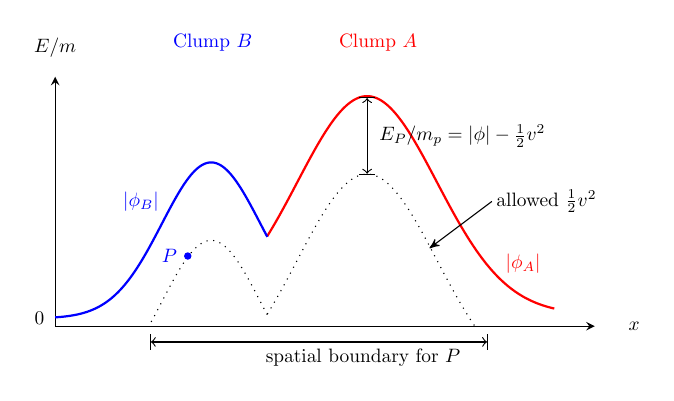
\begin{tikzpicture}[xscale=1,yscale=1,samples=400, transform shape,every node/.style={scale=0.7}]
	\begin{axis}[
		ticks=none,
		ymin=0,
		ymax=16,
		xmin=-8,
		xmax=26.6,
		axis x line=bottom,axis y line=left,
		%	axis lines = left,
		xlabel = $x$,
		ylabel = {$E/m$},
		legend pos=north west,
		every axis x label/.style={
			at={(ticklabel* cs:1.05)},
			anchor=west,
		},
		every axis y label/.style={
			at={(ticklabel* cs:1.05)},
			anchor=south,
		},
		axis equal image
	]
	
	% clump A
	\addplot [
		domain=5.58646:24, 
		samples=400, 
		color=red,thick
	] {14*exp(-(x-12)^2/40)+0.75};

%	\addplot [
%		domain=-10:5.58646, 
%		samples=400, 
%		color=red!10,thick,
%		style=dashed
%	] {14*exp(-(x-12)^2/40)+0.75};



	%clump B
%	\addplot [
%		domain=5.58:24, 
%		samples=400, 
%		color=blue!10, thick,
%		style=dashed
%	]{10*exp( (-(x-2)^2)/20)+0.5};

	\addplot [
		domain=-10:5.6, 
		samples=400, 
		color=blue, thick
	]{10*exp( (-(x-2)^2)/20)+0.5};
	
	
	
	%totalplot
%	\addplot [
%		domain=-10:24,
%		samples=400, 
%		color=violet, thick
%		]{10*exp( (-(x-2)^2)/20)+0.5 + 14*exp(-(x-12)^2/40)+0.75};
		
	%energy of P
	\addplot [
		domain=-10:5.6,
		samples=400, 
		color=black, dotted
	]{10*exp( (-(x-2)^2)/20)+0.5 - 5};
	\addplot [
		domain=5.6:24,
		samples=400, 
		color=black, dotted
	]{14*exp(-(x-12)^2/40)+0.75 - 5};
%	\addlegendentry{$\phi_A+\phi_B$}
	%
	%
	
	% Particles
%	\draw[darkgray] (100,100) circle (.1) node [left = .7mm] {$\alpha$};
%	\draw[cyan] (110,70) circle (.1) node [right = .7mm] {$\beta$};
%	\draw[purple] (105,45) circle (.1) node [left = .7mm] {$\gamma$};
%	\draw[teal] (92,25) circle (.1) node [left = .7mm] {$\beta$};
	\draw[blue, fill=blue] (105, 45) circle (.2) node [left = .7mm] {$P$};
%	\draw[|<->|, color=black] (80,20) -- node [right = 8mm, below=.1mm] {spatial boundary for $P$} (290,20) ;
	\draw[|<->|, color=black] (220,97) -- node [right = 1mm] {$E_P/m_p = |\phi| - \frac{1}{2}v^2$} (220,147);
	\draw[stealth'-, color=black] (260, 50) -- (300, 80);
	\node[] at (335, 80) {allowed $\frac{1}{2} v^2$};
%	\draw[|<->|,color=teal] (83,15) -- (117,15) node [right=1mm] {spatial boundary for $\beta$};


	%Naming
	\node[thick, blue] at (75,80) {$|\phi_B|$};
	\node[thick, red] at (320,40) {$|\phi_A|$};
%	\node[thick, violet] at (300,140) {$-\phi_{tot}=-(\phi_A+\phi_B)$};
%	\draw[color=black,style=dashed] (100+26.6584,25) -- (100+26.6584,120) node [above=1mm] {saddle};
	
	
	\end{axis};
	\node[] at (-0.2,0.1) {$0$};
	\node[thick, blue] at (2, 3.6) {Clump $B$};
	\node[thick, red] at (4.1, 3.6) {Clump $A$};
	
	\draw[|<->|, color=black] (1.2,-0.2) -- node [right = 8mm, below=.1mm] {spatial boundary for $P$} (5.5,-0.2) ;
	\end{tikzpicture}
\end{document}